\documentclass{article}
\usepackage[utf8]{inputenc}
\usepackage[spanish]{babel}
\usepackage{listings}
\usepackage{graphicx}
\usepackage{geometry}
\graphicspath{ {images/} }
\usepackage{cite}

\geometry{
textheight=23cm
}
\begin{document}

\begin{titlepage}
    \begin{center}
        \vspace*{0cm}
            
        \large
        \textbf{CLASES: PROYECTO FINAL}
            

        \vspace{8cm}
            
        \textbf{David Agudelo Ochoa}
        
        \vspace{0.5cm}
        
        \textbf{Erika Dayana León Quiroga}
            
        \vfill
            
        \vspace{0.8cm}
            
        \Large
        Universidad de Antioquia\\
        Despartamento de Ingeniería Electrónica y Telecomunicaciones\\
        Informática II\\
        Medellín-Antioquia\\
        Abril de 2021
            
    \end{center}
\end{titlepage}

\tableofcontents
\newpage
\section{Sección introductoria.}\label{intro}

En este informe se realizará la descripción de las clases que se implementarán para el desarrollo del proyecto final de la materia Informática II, esto nos permitirá planear el desarrollo de nuestro proyecto de manera que ya se tenga una idea general de este a la hora de iniciar con la codificación de nuestras clases. También nos ayudará a organizar mejor las ideas que tengamos para nuestro juego y estructurarlo de la mejor manera posible.

\section{Idea de juego.}\label{integrado}
El juego tratará de una madre lobo (nuestra heroína) quien intentará salvar a sus cachorros de la amenaza inminente del ser humano, el cual quiere apropiarse de los poderes sobrenaturales que los cachorros heredaron de su madre. Para esto iniciará una persecución en donde se enfrentará a los secuestradores de sus crías. Tendremos dos niveles de dificultad, en el primero nuestra heroína tendrá que esquivar proyectiles lanzados de manera rectilínea hacia ella, los cuales cambiarán su velocidad y frecuencia de aparición a medida que el tiempo avance, aumentando así la dificultad del mismo. Una vez superada esta primera etapa, el tipo de lanzamiento del proyectil cambiará, y se usará para este MOVIMIENTO PARABÓLICO y un SISTEMA FÍSICO ELÁSTICO (resorte, energía mecánica) el cual dará la velocidad inicial de los proyectiles en este nivel, la dificultad aumentará a medida que avance el nivel, cambiando la frecuencia de los proyectiles y su alcance máximo.
El último sistema físico requerido, se utilizará para la ambientación del juego y será MOVIMIENTO ARMÓNICO SIMPLE (un péndulo) en un reloj que muestre el tiempo restante del nivel actual.

\section{Descripción detallada del juego.}

Después de realizar la descripción detallada de las clases mostrando sus respectivos métodos y atributos, continuaremos con una explicación de cómo serán utilizadas estas clases dentro del juego. También se describirán los escenarios a utilizar y los objetos que harán parte de estos.

Tal como se mencionó en la sección \textbf{Idea de juego}, nuestra \textbf{Héroe} será una loba con poderes supernaturales, la cual vive tranquilamente con sus crías hasta que son raptadas por un grupo de humanos, cuyos intereses se centran en apropiarse de los poderes que tienen los cachorros, tal como ha hecho durante años con todo lo que nos brinda la naturaleza.

\begin{figure}[h]
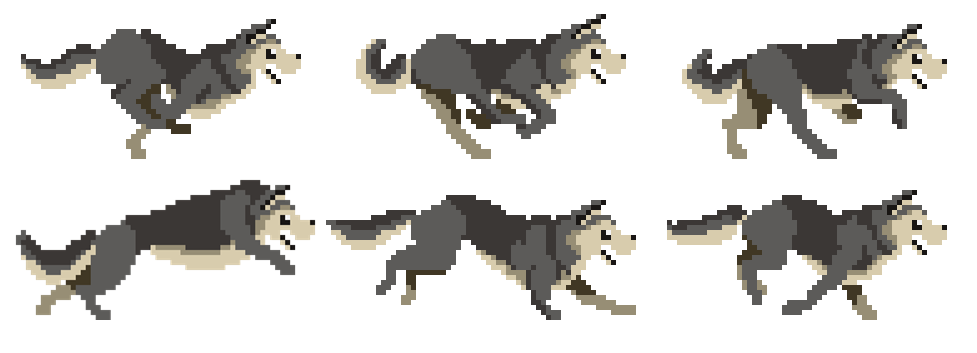
\includegraphics[scale=0.7]{Images/spriteheroe.png}
\centering
\caption{Sprite que se usará para animar a nuestro héroe .}
\label{fig:spriteheroe}
\end{figure}

Tras este desafortunado incidente, nuestra \textbf{Héroe} emprenderá una persecución para poder rescatar a sus cachorros, sin embargo este asedio no será un camino fácil, pues no sabe a qué tendrá que enfrentarse.



En nuestro primer escenario (\textbf{Nivel-1}), el \textbf{Héroe} perseguirá un auto de policía (\textbf{Enemigo}) que trata de escapar después de capturar a los cachorros en el bosque donde la familia de lobos se encontraba viviendo tranquilamente. Pero este \textbf{Enemigo} no se limitará a huir simplemente, sino que además estos cobardes recurrirán a disparos de balas (\textbf{Proyectil}) con intención de herir, o incluso matar a nuestra Madre preocupada. Para evitar estos ataques, tendrá que recurrir a grandes saltos, mientras corre a altas velocidades para así evitar hacerse daño y no perder de vista a los secuestradores de sus hijos.

\begin{figure}[h]

\includegraphics[scale=0.7]{Images/spriteproyectil.png}
\centering
\caption{Sprite del proyectil para el nivel uno.}
\label{fig:spriteproy}
\end{figure}

Dado que el auto de policía alcanza velocidades demasiado elevadas, nuestra heroína debe limitarse a no perderlos de vista, y seguirles el rasto hasta su lugar de destino. Por lo que deberá aguantar un tiempo (\textbf{Reloj}) de 120 segundos esta intensa persecución.

\begin{figure}[h]
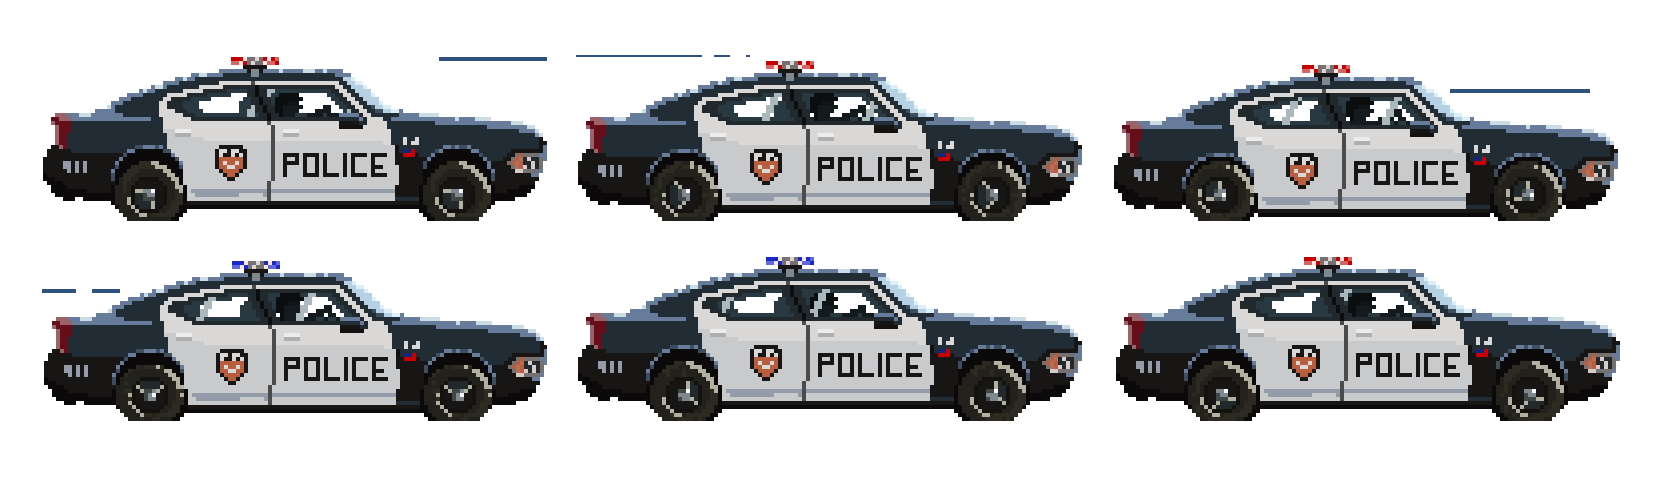
\includegraphics[scale=0.4]{Images/spritecarro.png}
\centering
\caption{Sprite del enemigo del nivel uno.}
\label{fig:spriteproy}
\end{figure}


Si consigue su cometido, el carro de policía \textbf{Enemigo}, tendrá que recurrir a entes mayores ante la imposibilidad de detener a nuestra loba. Por lo que ingresará a una base en busca de ayuda, y de poder dificultar el rescate de los cachorros. 

\vspace{5mm}

Es aquí donde ocurre nuestro segundo escenario (\textbf{Nivel-2}), en donde nuestra heroína se encontrará con un gran tanque (\textbf{Enemigo}), el cuál a pesar de compartir intenciones con nuestro anterior \textbf{Enemigo}, que son el transportar a los cachorros y detener a su madre, este tendrá un poder bélico de un nivel completamente distinto, pues lanzará los proyectiles imitando el tiro de un cañón y su alcance será desconocido para nuestra héroe, la velocidad de salida del proyectil será diferente en cada tiro y se calculará haciendo uso de teoría de resortes, pues se relacionará con la compresión aleatoria que se le realice al resorte modelado para nuestro juego. Para hacerle frente, nuestra loba tendrá que usar aquellos poderes por los cuales la buscan. Usará su ultravelocidad con teletransportación para poder evitar estos proyectiles (\textbf{Proyectil}), ya que no bastará un simple salto.

\newpage
\begin{figure}[h]
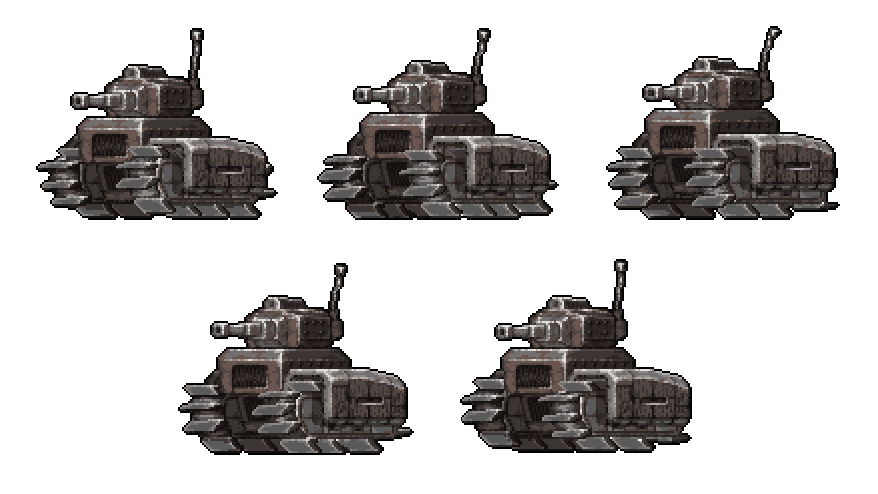
\includegraphics[scale=0.7]{Images/spritetanque.png}
\centering
\caption{Sprite del enemigo del nivel dos.}
\label{fig:spriteproy}
\end{figure}

Nuevamente, nuestra heroína tratará de alcanzar a nuestro enemigo para recuperar sus crías, por lo que este, además de atacarla, deberá desplazarse con rapidez, pero dado que este no está diseñado para alcanzar velocidades tan altas, estará sobreesforzando su maquinaria, por lo que tendrá un tiempo de 120 segundos hasta que su sistema falle por completo. Si nuestra heroína aguanta hasta que la maquinaria falle, podrá recuperar a sus cachorros, y volver a vivir pacíficamente en el bosque.

\section{Clases.}
Para la creación de los mapas mentales que nos ayudarán con la estructuración de las clases, se utilizará el siguiente código de color: Verde para las clases, amarillo para las clases abstractas, blanco para los atributos, azul para los métodos y morado para los métodos abstractos.

\begin{figure}[h]
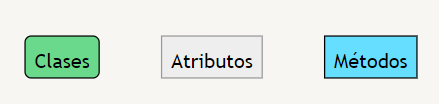
\includegraphics[scale=0.8]{Images/colores.png}
\centering
\caption{Código de color para los mapas mentales.}
\label{fig:codigo}
\end{figure}

\subsection{ObjetoAnimado.}\label{objeto_animado}
\begin{itemize}
  \item \textbf{Atributos:} En esta clase Objeto animado, tendremos como atributos la posición (x,y), el tamaño y número de frames el cual es necesario para realizar la animación de los objetos.
  
  \item \textbf{Métodos:} En los métodos tenemos Animar, en donde se actualizarán los frames de los objetos que queramos animar cada cierto tiempo, para esto se necesitarán dos parámetros, el número de frames de la animación y el path de cada una de las imágenes para crear la animación completa, para obtener este último parámetro se utilizará el retorno del método stringPath el cual nos ayudará a contruir el nombre de la dirección del archivo dependinedo del número de frame.
\end{itemize}

\newpage
\begin{figure}[h]
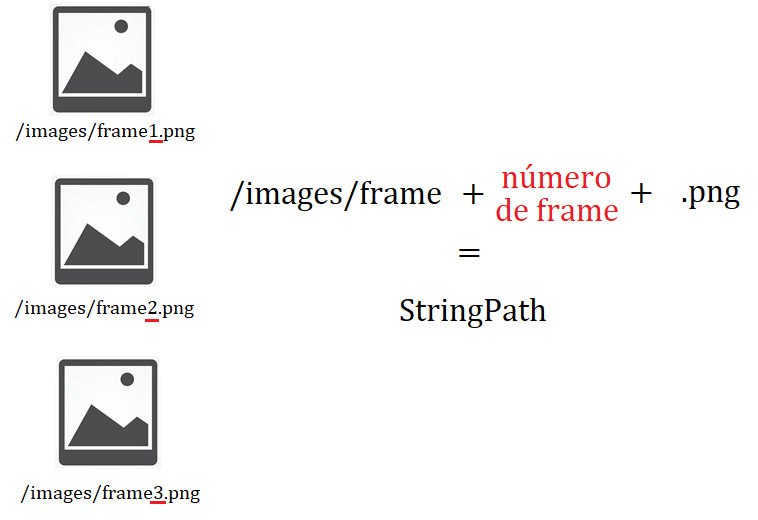
\includegraphics[scale=0.6]{Images/string.png}
\centering
\caption{Ejemplo del funcionamiento del método stringPath. Como podemos ver, la primera y última parte del string se mantiene constante mientras que el número de frame va cambiando para lograr la animación de los objetos presentes en la escena.}
\label{fig:string}
\end{figure}

\begin{figure}[h]
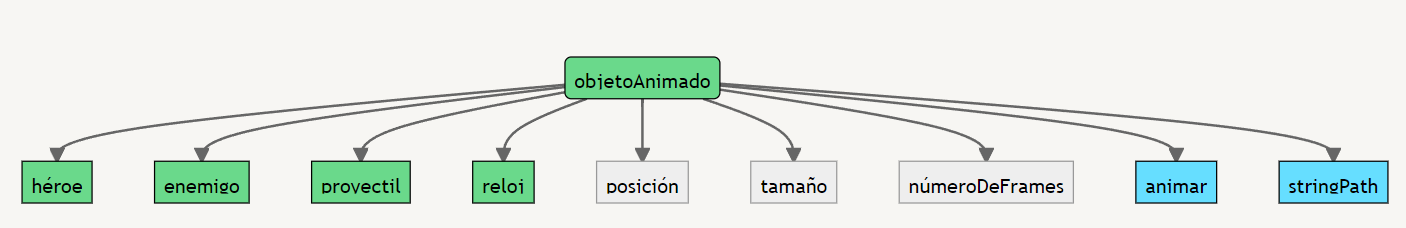
\includegraphics[scale=0.5]{Images/ObjetoAnimado.png}
\centering
\caption{Mapa mental de la clase objetoAnimado.}
\label{fig:mmobjani}
\end{figure}

    \subsubsection{Héroe}
    \begin{itemize}
        \item \textbf{Atributos:} Dentro los atributos de la clase Héroe encontraremos el número de vidas, si el héroe dispone de su poder en un nivel determinado y por último el nivel en el que se encuentra.
        \item \textbf{Métodos:} Tendremos dos métodos, la actualización de la posición del héroe en Y cuando este realice un salto, y la verificación de la colisión del héroe con los límites del escenario.
    \end{itemize}
    
    \subsubsection{Enemigo}
    \begin{itemize}
        \item \textbf{Atributos:} Esta clase tendrá un único atributo que cambiará el nivel de dificultad dentro de un mismo nivel a medida que avance el tiempo.
    \end{itemize}
    
\begin{figure}[h]
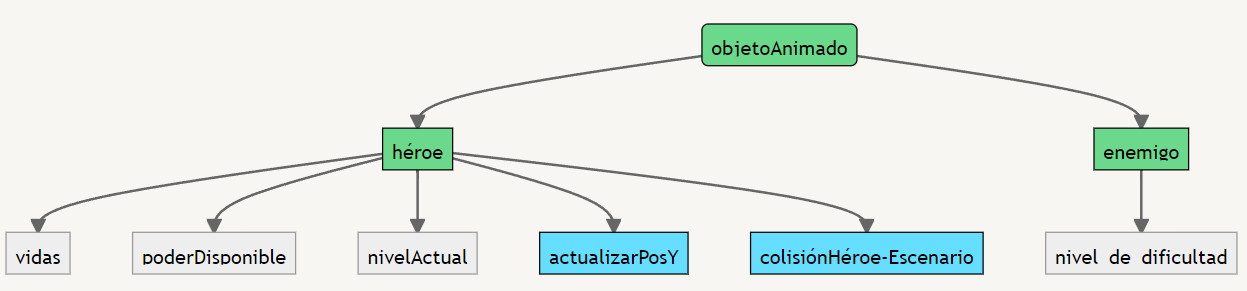
\includegraphics[scale=0.5]{Images/Heroe-enemigo.png}
\centering
\caption{Mapa mental de la clase héroe y de la clase enemigo.}
\label{fig:mmheroe}
\end{figure}
    
    \subsubsection{Proyectil}
    \begin{itemize}
        \item \textbf{Atributos:} En este caso tendremos de atributos la velocidad inicial del  proyectil y la frecuencia de aparición de este.
        \item \textbf{Métodos:} Dentro de los métodos encontraremos la verificación de la colisión entre el proyectil y el héroe, también la colisión entre el proyectil y los límites del escenario, la descripción del movimiento (MRU) usado para el proyectil en el nivel 1, y por último un método que describa el movimiento de tiro parabólico con resorte utilizado para el proyectil del nivel 2. 
    \end{itemize}
    
\begin{figure}[h]
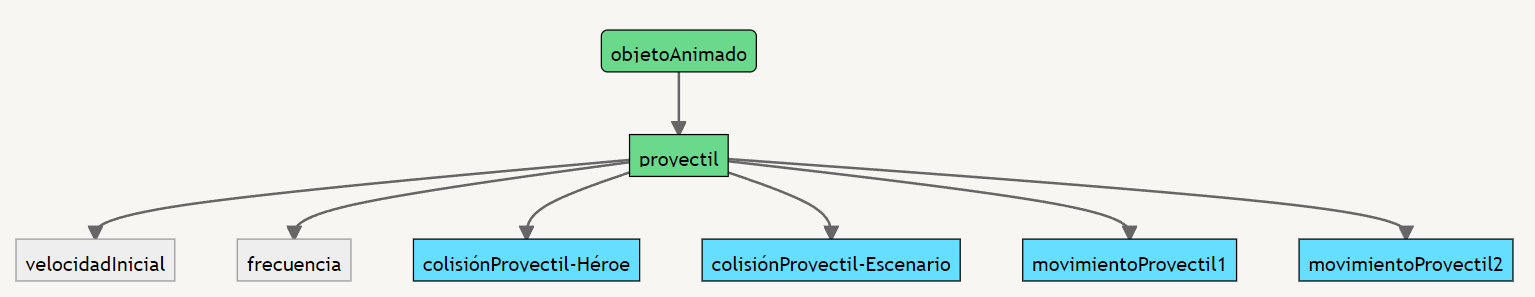
\includegraphics[scale=0.5]{Images/proyectil.png}
\centering
\caption{Mapa mental de la clase proyectil.}
\label{fig:mmproy}
\end{figure}
    
    
    \subsubsection{Reloj}
    \begin{itemize}
        \item \textbf{Atributos:} Tendrá un atributo que nos permitirá llevar la cuenta del tiempo de la partida.
        \item \textbf{Métodos:} Tendremos un método que nos permitirá modelar el movimiento de un péndelo de reloj, el cual hará parte de la ambientación del juego. También se necesitará otro método para actualizar la visualización del tiempo de juego.
    \end{itemize}
    
    
\begin{figure}[h]
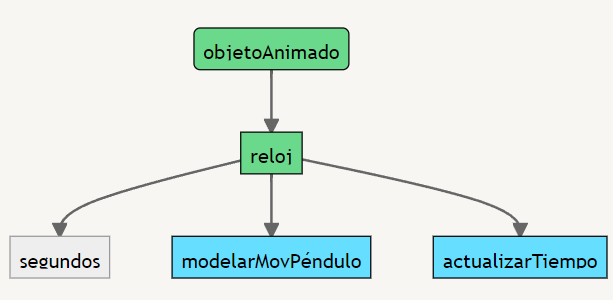
\includegraphics[scale=0.8]{Images/reloj.png}
\centering
\caption{Mapa mental de la clase reloj.}
\label{fig:mmreloj}
\end{figure}


\subsection{Nivel.}\label{niveles}
Para la clase nivel se decidió que fuese de tipo abstracto, pues posee métodos que cambiarán dependiendo de las clases que los hereden.
\begin{itemize}
  \item \textbf{Atributos:} La clase Niveles tendrá como único atributo el timepo de duración del nivel.
  
  \item \textbf{Métodos:} Tendremos el método para guardar el nivel, el cual nos ayudará a almacenar datos importantes del nivel actual, como la posición del héroe, las vidas de este, el tiempo restante de partida, nivel de dificultad y nivel en el que se encuentra.
  
  \item \textbf{Métodos abstractos:}  Con respecto a los métodos abstractos, tendremos uno que nos permitirá iniciar el nivel correspondiente desde cero, creando los objetos para el funcionamiento del mismo y por último, el método para cargar el nivel guardado, el cual se encargará de tomar los datos guardados y recrear el nivel partiendo de estos. 
  
\end{itemize}

\begin{figure}[h]
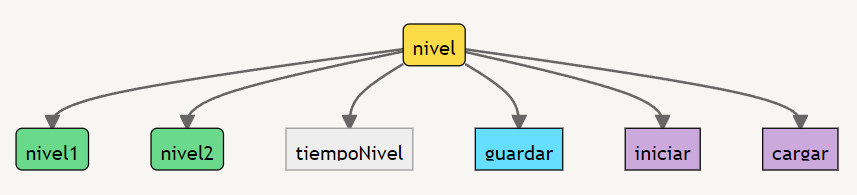
\includegraphics[scale=0.8]{Images/niveles.png}
\centering
\caption{Mapa mental de la clase niveles.}
\label{fig:mmniveles}
\end{figure}

    \subsubsection{Nivel-1}
    \begin{itemize}
        \item \textbf{Métodos:} El método iniciar instanciará los objetos necesarios para la creación del nivel 1, dependiendo de las características de este. Para el método cargar se utilizarán los datos almacenados con ayuda del método guardar y de esta forma retomar el nivel en el punto guardado.
    \end{itemize} 
    
    \subsubsection{Nivel-2}
    \begin{itemize}
        \item \textbf{Métodos:} El método inciar instanciará los objetos necesarios para la creación del nivel 2, dependiendo de las características de este. Para el método cargar, se utilizarán los datos almacenados con ayuda del método guardar y de esta forma retomar el nivel en el punto guardado.
    \end{itemize}
    

\section{Conclusiones.}
    \begin{itemize}
        \item El proceso de estructurar las clases sin desarrollar código es bastante complejo, pues todo parte mucho de la especulación, ya que no hay garantías de si lo que se planeó podrá implementarse de manera exitosa.
        
        \item A pesar del comentario del ítem anterior, una vez alcanzamos un buen porcentaje de clases definidas, nos dimos cuenta de la simplicidad que adquiere la estructuración, pues nos garantiza que más adelante, una vez se empiece a codificar, exista una buena organización de las clases y una correcta descripción de sus métodos y atributos.
        
        \item El trabajo en equipo hace más ameno el desarrollo de los proyectos, y a pesar de que a veces puedan haber desacuerdos, mientras haya buena comunicación, no hay problema que no pueda solucionarse.
    \end{itemize}
    
    \vspace{10mm}
    
\textbf{NOTA:} Los sprites utilizados en este proyecto se tomaron de: http://www.animated-gifs.fr/animated-gifs.php y serán usados únicamente con fines acedémicos sin ninguna retribución económica.


\end{document}
